\documentclass{article}
\usepackage{graphicx}
\usepackage{amsmath}
\usepackage{array}
\usepackage{fancyhdr}
\usepackage{amssymb}
\usepackage[shortlabels]{enumitem}
\usepackage{tikz}
\usepackage{subfigure}
\usepackage{hyperref}
\usepackage{optidef}

\usetikzlibrary{arrows.meta}

\DeclareMathOperator{\R}{\mathbb R}

\pagestyle{fancy}
\fancyhead[L]{Banghao Chi}
\fancyhead[C]{Homework 7}
\fancyhead[R]{18th Apr}

\fancyfoot[C]{\thepage}

\renewcommand{\headrulewidth}{0.5pt}
\renewcommand{\footrulewidth}{0.5pt}

\newcommand{\Z}{\mathbb{Z}}
\newcommand{\Q}{\mathbb{Q}}
\newcommand{\C}{\mathbb{C}}
\newcommand{\F}{\mathbb{F}}
\newcommand{\N}{\mathbb{N}}
\newcommand{\real}{\textrm{Re }}
\newcommand{\imag}{\textrm{Im }}

\begin{document}

\begin{enumerate}

    \item[1.] The diagram below gives a residual graph for a network. (Black edges are ``forward'' edges, red edges are ``backward'' edges.)

    \begin{center}
        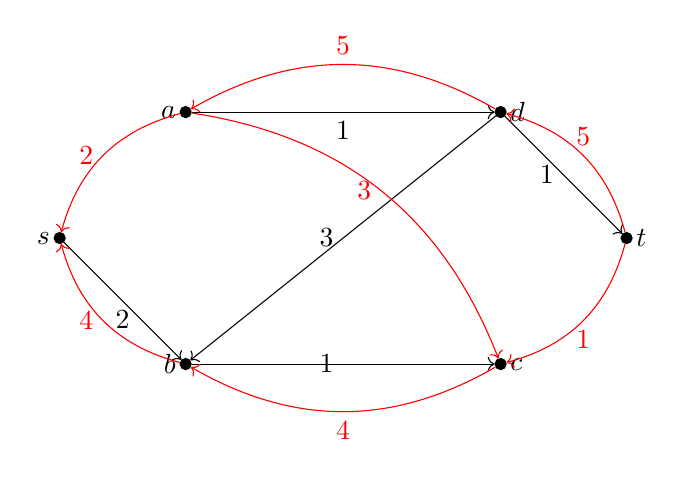
\begin{tikzpicture}[scale=0.8]
            \node[circle,fill=black,draw,inner sep=0pt,minimum size=4pt] (d) at (5, 2) {};
            \node[circle,fill=black,draw,inner sep=0pt,minimum size=4pt] (a) at (0, 2) {};
            \node[circle,fill=black,draw,inner sep=0pt,minimum size=4pt] (s) at (-2, 0) {};
            \node[circle,fill=black,draw,inner sep=0pt,minimum size=4pt] (b) at (0, -2) {};
            \node[circle,fill=black,draw,inner sep=0pt,minimum size=4pt] (c) at (5, -2) {};
            \node[circle,fill=black,draw,inner sep=0pt,minimum size=4pt] (t) at (7, 0) {};
    
            \node[anchor=west] at (d) {$d$};
            \node[anchor= east] at (a) {$a$};
            \node[anchor=east] at (s) {$s$};
            \node[anchor=east] at (b) {$b$};
            \node[anchor= west] at (c) {$c$};
            \node[anchor=west] at (t) {$t$};
    
            \draw[->] (a) edge node[midway,below,minimum size=4pt] {$1$} (d) 
            (d) edge node[midway,left,minimum size=4pt] {$1$} (t)
            (d) edge node[midway,left,minimum size=4pt] {$3$} (b)
            (s) edge node[midway,below,minimum size=4pt] {$2$} (b)
            (b) edge node[midway,left,minimum size=4pt] {$1$} (c);

            \draw[->, red] (b) edge[bend left] node[midway,left,minimum size=4pt] {$4$} (s) 
            (a) edge[bend right] node[midway,left,minimum size=4pt] {$2$} (s)
            (d) edge[bend right] node[midway,above,minimum size=4pt] {$5$} (a)
            (t) edge[bend right] node[midway,above,minimum size=4pt] {$5$} (d)
            (t) edge[bend left] node[midway,below,minimum size=4pt] {$1$} (c)
            (a) edge[bend left] node[midway,left,minimum size=4pt] {$3$} (c)
            (c) edge[bend left] node[midway,below,minimum size=4pt] {$4$} (b);
        \end{tikzpicture}
    \end{center}


    \begin{enumerate}[(a)]
        \item Determine the original network and capacities.

        \item Find the flow which produces this residual graph.

        \item Find a cut with the same capacity as the value of this flow.
    \end{enumerate}

    \textbf{Solution:} \\

    \begin{enumerate}[(a)]
\item Original capacities  
\[
s\to a:2,\; s\to b:6,\; a\to d:6,\; d\to t:6,\;
d\to b:3,\; b\to c:5,\; c\to a:3,\; c\to t:1 .
\]

\item A feasible flow that yields the given residual graph can be found using all backward edges:
\begin{align*}
f(s,a)&=2, & f(s,b)&=4,\\
f(a,d)&=5, & f(d,t)&=5,\\
f(d,b)&=0, & f(b,c)&=4,\\
f(c,a)&=3, & f(c,t)&=1.
\end{align*}
The value of the flow is \( |f| = 6 \).

\item A cut having the same capacity  
Take \( S=\{s,b,c\} \) and \( T=\{a,d,t\} \).  
The forward edges from \( S \) to \( T \) are
\[
s\to a,\; c\to a,\; c\to t
\]
with total capacity
\[
2+3+1 = 6 = |f|.
\]
Hence the cut capacity equals the flow value.
\end{enumerate}

    \newpage
    
    \item[2.] Consider the following matching (that is, $M = \{(a, d),(b, e)\}$) in a bipartite graph:
    
    \begin{center}
        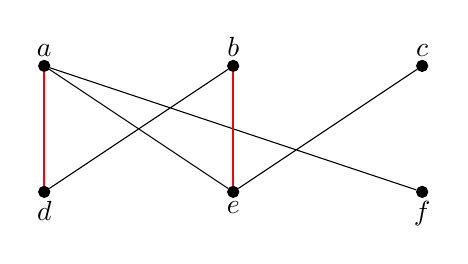
\begin{tikzpicture}[scale=0.8]
            \node[circle,fill=black,draw,inner sep=0pt,minimum size=4pt] (a) at (0, 2) {};
            \node[circle,fill=black,draw,inner sep=0pt,minimum size=4pt] (b) at (3, 2) {};
            \node[circle,fill=black,draw,inner sep=0pt,minimum size=4pt] (c) at (6, 2) {};
            \node[circle,fill=black,draw,inner sep=0pt,minimum size=4pt] (d) at (0, 0) {};
            \node[circle,fill=black,draw,inner sep=0pt,minimum size=4pt] (e) at (3, 0) {};
            \node[circle,fill=black,draw,inner sep=0pt,minimum size=4pt] (f) at (6, 0) {};
    
            \node[anchor=south] at (a) {$a$};
            \node[anchor=south] at (b) {$b$};
            \node[anchor=south] at (c) {$c$};
            \node[anchor=north] at (d) {$d$};
            \node[anchor=north] at (e) {$e$};
            \node[anchor=north] at (f) {$f$};
    
           \draw (e) -- (a) -- (f) (b) -- (d) (c) -- (e);

            \draw[thick, red] (a) -- (d) (b) -- (e);
        \end{tikzpicture}
    \end{center}

    First, convert this matching into a feasible flow in a network. Then, find an augmenting path in that network, and use it to improve the matching to a larger one.

    \textbf{Solution:}
\begin{itemize}
    \item Source \(s\) connects to every \(u\in L=\{a,b,c\}\) with capacity \(1\).
    \item Every \(v\in R=\{d,e,f\}\) connects to the sink \(t\) with capacity \(1\).
    \item For each edge \((u,v)\) in the bipartite graph add the arc \(u\to v\) with capacity \(\infty\):
          \[
          a\to d,\; a\to f,\; b\to d,\; b\to e,\; c\to e .
          \]
\end{itemize}

For feasible flow, we can let:
\begin{align*}
f(s,a)&=1, & f(a,d)&=1, & f(d,t)&=1,\\
f(s,b)&=1, & f(b,e)&=1, & f(e,t)&=1,\\
f(\text{all other arcs})&=0.
\end{align*}

The value of the above flow equals \(2\), matching the size of \(M\).

Arcs that carry flow \(1\) acquire a backward arc of capacity \(1\), while unsaturated arcs keep their forward capacity.
In this residual network an \(s\!-\!t\) path exists:
\[
s\to c\to e\to b\to d\to a\to f\to t,
\]
whose residual capacity is \(1\).

Augment one unit along that path.  
Non-zero left-to-right flows after augmentation are
\[
f(a,f)=1,\qquad
f(b,d)=1,\qquad
f(c,e)=1.
\]

Hence the new matching is
\[
M'=\{(a,f),\,(b,d),\,(c,e)\},
\]
with size \(3>2\), so the matching has been successfully improved.

    \newpage

    \item[3.] Write down a linear program for a general feasible circulation problem. (There is no objective function, so make the objective function just ``maximize 0''.)
    Then, take the dual of this linear program.

    \textbf{Solution:} \\

Primal linear program: feasible circulation
\begin{align*}
\text{maximize } & 0 \\[6pt]
\text{s.t. } 
& \sum_{e \in \delta^{+}(v)} f_e \;-\; \sum_{e \in \delta^{-}(v)} f_e \;=\; 0 && v \in V \\[4pt]
& l_e \;\le\; f_e \;\le\; u_e && e \in E
\end{align*}

Dual linear program
\begin{align*}
\text{minimize } & \sum_{e \in E} \bigl(u_e \,\alpha_e \;-\; l_e \,\beta_e\bigr) \\[6pt]
\text{s.t. } 
& \pi_v \;-\; \pi_w \;+\; \alpha_e \;-\; \beta_e \;=\; 0 && e = (v,w) \in E \\[4pt]
& \alpha_e \;\ge\; 0 && e \in E \\[2pt]
& \beta_e \;\ge\; 0 && e \in E
\end{align*}

    \newpage

    \item[4.] Let $(N, A)$ be an instance of the supply-and-demand version of max flow with capacities $c$ and demands $d$. Recall the max-flow reduction from lecture. Prove that there is a feasible flow if and only if the optimal solution in the max-flow reduction saturates all arcs leaving $s$ and entering $t$ (an arc is saturated if the flow along it is equal to its capacity).

    \textbf{Solution:} \\



    \newpage

    \item[5.] Consider the minimum-cost flow problem given in the first diagram below. The spanning tree shown in the second diagram gives a basic feasible solution.

    \begin{figure}[h]
    \centering
        \begin{subfigure}
            \centering
            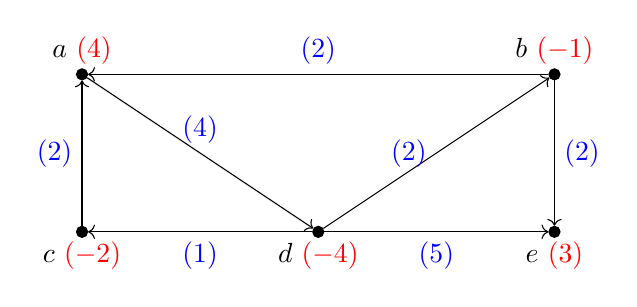
\begin{tikzpicture}
                \node[circle,fill=black,draw,inner sep=0pt,minimum size=4pt] (a) at (0, 2) {};
                \node[circle,fill=black,draw,inner sep=0pt,minimum size=4pt] (b) at (6, 2) {};
                \node[circle,fill=black,draw,inner sep=0pt,minimum size=4pt] (c) at (0, 0) {};
                \node[circle,fill=black,draw,inner sep=0pt,minimum size=4pt] (d) at (3, 0) {};
                \node[circle,fill=black,draw,inner sep=0pt,minimum size=4pt] (e) at (6, 0) {};

                \node[anchor=south] at (a) {$a$ {\textcolor{red}{$(4)$}}};
                \node[anchor=south] at (b) {$b$ {\textcolor{red}{$(-1)$}}};
                \node[anchor=north] at (c) {$c$ {\textcolor{red}{$(-2)$}}};
                \node[anchor=north] at (d) {$d$ {\textcolor{red}{$(-4)$}}};
                \node[anchor=north] at (e) {$e$ {\textcolor{red}{$(3)$}}};

                \draw[->] (a) edge node[midway,above,minimum size=4pt] {\textcolor{blue}{$(4)$}} (d)
                (b) edge node[midway,above,minimum size=4pt] {\textcolor{blue}{$(2)$}} (a)
                (b) edge node[midway,right,minimum size=4pt] {\textcolor{blue}{$(2)$}} (e)
                (c) edge node[midway,left,minimum size=4pt] {\textcolor{blue}{$(2)$}} (a)
                (d) edge node[midway,below,minimum size=4pt] {\textcolor{blue}{$(1)$}} (c)
                (d) edge node[midway,left,minimum size=4pt] {\textcolor{blue}{$(2)$}} (b)
                (d) edge node[midway,below,minimum size=4pt] {\textcolor{blue}{$(5)$}} (e);
            \end{tikzpicture}
        \end{subfigure}%
        \qquad%
        \begin{subfigure}
            \centering
            \begin{tikzpicture}
                \node[circle,fill=black,draw,inner sep=0pt,minimum size=4pt] (a) at (0, 2) {};
                \node[circle,fill=black,draw,inner sep=0pt,minimum size=4pt] (b) at (6, 2) {};
                \node[circle,fill=black,draw,inner sep=0pt,minimum size=4pt] (c) at (0, 0) {};
                \node[circle,fill=black,draw,inner sep=0pt,minimum size=4pt] (d) at (3, 0) {};
                \node[circle,fill=black,draw,inner sep=0pt,minimum size=4pt] (e) at (6, 0) {};

                \node[anchor=south] at (a) {$a$};
                \node[anchor=south] at (b) {$b$};
                \node[anchor=north] at (c) {$c$};
                \node[anchor=north] at (d) {$d$};
                \node[anchor=north] at (e) {$e$};

                \draw[->] (b) edge (a) (c) edge (a) (d) edge (b) (d) edge (e);
            \end{tikzpicture}
        \end{subfigure}
    \end{figure}

    \begin{enumerate}[(a)]
        \item Solve for the flows along each of the arcs in the basic feasible solution given by this spanning tree.

        \item Determine the reduced cost of each of the nonbasic arcs in the network, then do a single pivoting step.
        
    \end{enumerate}

    \textbf{Solution:} \\


    
\end{enumerate}

\end{document}